\documentclass[10pt, conference]{IEEEtran}
\usepackage{cite}
\usepackage{url}
\usepackage{amsmath,amssymb,amsfonts}
\usepackage{algorithmic}
\usepackage{graphicx}
\usepackage{textcomp}
\usepackage{xcolor}
\usepackage{listings}
\usepackage{svg}
\usepackage{placeins}

\graphicspath{{./images/}}

% Go Code Formatting Setup
\lstset{
	language=Go,
	basicstyle=\ttfamily\footnotesize,
	keywordstyle=\color{blue},
	commentstyle=\color{green!60!black},
	stringstyle=\color{purple},
	breaklines=true,
	frame=single
}

\begin{document}
	
	\title{Implementation of a Basic Blockchain with PoW and Merkle Patricia Tries}
	
	\author{\IEEEauthorblockN{Joel González Jiménez}
		\IEEEauthorblockA{Universitat Politècnica de Catalunya – FIB\\
			Barcelona, Spain \\
		}
	}
	
	\maketitle
	
	\begin{abstract}
	Blockchain research is continually driving new functionalities and optimizations. As a result, modern blockchains look vastly different from the beginning. This paper presents a modular, localhost blockchain prototype written in Go, specifically engineered to study the core concepts such as consensus mechanisms, Proof-of-Work (PoW), and cryptografic proofs with modified hexary Merkle Patricia Trie (MPT). By decoupling these pillars from the overhead of peer-to-peer networking, we purpose a solid framework built from scratch for newcomers understand better the foundations of blockchain systems. Also debugging tools and tests are provided to facilitate building on top more functionalities and further optimizations. Crucially, we leverage some changes and systemic constraints of a MPT implementation that utilizes self-referential content-addressed hashing to achieve more efficient space usage.
	\end{abstract}
	
	\begin{IEEEkeywords}
		Blockchain, Merkle Patricia Trie, Proof of Work, Cryptographic Proof.
	\end{IEEEkeywords}
	
	\section{Introduction}
	Blockchain research is continually driving new functionalities and optimizations. As a result, modern blockchains look vastly different from the beginning. While early distributed networks relied strictly on simple transaction sequences appended to linear ledgers, contemporary platforms require fine-grained state tracking and highly optimized authenticated storage configurations. 
	
	This project is a hands-on implementation of an experimental blockchain environment designed to deliberately isolate and study these core foundational subsystems, focusing comprehensively on:
	\begin{itemize}
		\item \textbf{Consensus Mechanism (PoW):} The throttling of ledger updates through intensive algorithmic resource consumption, provided by Bitcoin \cite{nakamoto2008bitcoin}.
		\item \textbf{Merkle Patricia Trie (MPT):} The design of an authenticated, radix-based data organization layer capable of emitting cryptographic proofs, provided by Ethereum \cite{wood2014ethereum}.
	\end{itemize}
	
	The entire implementation and code can be found available in the open github repository \cite{jowy-ti_dsproject}.
	
	\section{Related Work}
	
	The landscape of blockchain research can be overwhelming, to bypass the steep learning curves and noise of complex codebases like Go-Ethereum (Geth), researchers frequently rely on lightweight blockchain frameworks. This frameworks are very useful because can be used to extend functionalities and provide optimizations without making from scratch your own blockchain system.
	
	Minimalist educational implementations, such as \textit{Naivechain}\cite{hartikka} or early Hyperledger prototypes, provide clean environments to study consensus loops but frequently strip away complex world-state tracking, substituting a proper MPT with basic flat arrays or simple cryptographic hash chains.  This project bridges this gap by retaining a functionally rigorous, hexary MPT layout and a resource-intensive PoW mining loop, while stripping away the unpredictable latency of P2P network layers to allow direct, deterministic profiling of state integrity.
	
	\section{Core System Capabilities}
	The developed platform provides a robust research testbed that successfully demonstrates four primary system capabilities:
	\begin{itemize}
		\item \textbf{Cryptographic Immutability:} Enforcing absolute historical integrity across the ledger via sequential SHA-256 block-hashing tied directly to the execution bounds of the Proof-of-Work consensus loop.
		\item \textbf{Lightweight Verification:} Utilizing a custom Merkle Patricia Trie layout to yield deterministic cryptographic execution proofs, maintaining an efficient operational lookup bounds of $\mathcal{O}(\log n)$.
		\textmu \item \textbf{Persistent State Storage:} Implementing a reliable underlying data-store layer utilizing a database to preserve the entire blockchain structure across successive experimental runs.
		\item \textbf{Debugging Tools and Tests:} Integrating diagnostic utilities and localized test suites optimized for analyzing the serialization size, runtime growth, and data density of individual block payloads.
	\end{itemize}
	
	\section{Custom Merkle Patricia Trie Design}
	The data storage architecture modifies the traditional execution parameters of a standard Merkle Patricia Trie to optimize for a per-block data log environment.
	
	\subsection{Architectural Departures from Standard MPT}
	Unlike generalized global world-state implementations (such as Ethereum), this framework enforces four explicit structural constraints:
	\begin{enumerate}
		\item \textbf{GOB Encoding Framework:} The system substitutes standard Recursive Length Prefix (RLP) \cite{wood2014ethereum} serialization for Go's native \texttt{GOB} \cite{gob} binary encoder to natively streamline abstract interface across node variations.
		\item \textbf{Value-Free Branch Nodes:} Standard MPT branch nodes store a terminating value slot to accommodate variable-length paths. In this framework, \textbf{Branch nodes do not contain a value} field because every key in the sub-tree shares a strictly uniform static length constraint.
		\item \textbf{Self-Referential Content Addressing:} The path/key utilized to navigate to a value inside the trie is uniquely derived as the SHA-256 hash of the target value itself:
		$$\text{Path} = \text{SHA256}(\text{Value})$$
		Consequently, every key mapping to a node spans exactly 32 bytes (64 hexary nibbles), eliminating path variance.
	\end{enumerate}
	
	\subsection{Node Structural Layouts}
	An example of the structure implemented Merkle Patricia Trie can be seen in Figure \ref{fig:MPT} . There are three different variations of a \texttt{Node}:
	
	\begin{itemize}
		\item \textbf{Leaf Node:} Contains the terminal path slice directly to its corresponding raw data payload.
		\item \textbf{Branch Node:} Is an array of 16 slot hashes (\texttt{Childs\_hash [16][32]byte}) to manage routing through nibles.
		\item \textbf{Extension Node:} Leverages path compression by squashing a sequence of shared nibbles (\texttt{Path\_shared}) and contains a reference of the next hash (\texttt{Next\_hash}).
	\end{itemize}
	
	\begin{figure}[htbp]
		\centering
		\includesvg[width=1\linewidth]{MPT.svg}
		\caption{Custom hexary Merkle Patricia Trie}
		\label{fig:MPT}
	\end{figure}
	
	\section{Serialization Analysis: GOB vs. RLP}
	A foundational design trait of this prototype is its reliance on Go's internal binary encoder (\texttt{GOB}) instead of the Recursive Length Prefix (\texttt{RLP}).
	
	\subsection{The GOB Rationale}
	GOB provides exceptional utility inside a specialized, single-language Go prototype. It inherently processes abstract interface schemas. By embedding type descriptions and metadata definitions directly inside the resulting byte array, it allows the storage layer to seamlessly serialize and deserialize abstract \texttt{Node} definitions without requiring manual byte-parsing and validation boilerplates.
	
	\subsection{The RLP Consensus Imperative}
	While optimal for a localized framework, GOB is critically flawed in distributed multi-node consensus environments because it lacks absolute binary determinism. Internal stream optimizations and compiler variant updates can yield subtle discrepancies in output byte arrays from identical input data, causing irreversible ledger forks. Implementing \textbf{RLP} represents a vital optimization upgrade for production deployment; RLP omits all struct type schema data, encoding exclusively lengths and raw bytes to ensure absolute cross-client cryptographic determinism.
	
	\section{Consensus Engine: Proof-of-Work}
	To commit an assembled data block securely to the persistent ledger, the mining module (\texttt{pow.go}) forces computational verification. 
	
	\subsection{Target Boundary Evaluation}
	A block's validity is governed by a strict mathematical constraint. The system boundary target big integer $T$ is calculated by executing a left-shift operation against a baseline value based on a globally declared block difficulty variable $D$:
	\begin{equation}
		T = 1 \ll (\text{HashLength} - \text{Difficulty})
	\end{equation}
	Where $\text{HashLength}$ represents the bit-width of the cryptographic hashing output space (256 bits).
	
	\subsection{The Execution Loop}
	The consensus engine loops through individual incrementing iterations of a block's 64-bit integer \texttt{Nonce} field, validating that the resulting double-pass hash satisfies the inequality:
	\begin{equation}
		\text{SHA256}(\text{BlockData} \parallel \text{Nonce}) < T
	\end{equation}
	Once a nonce is discovered that results in a hash of the block with an integer value below the calculated target line $T$, the mining cycle terminates, and the block is broadcast to the storage management layer.
	
	\section{Architectural Design}
	The architectural design strictly prioritizes modularity, enforcing a highly structured, acyclic dependency graph among the application classes to clearly assign operational responsibilities, Figure \ref{fig:class_diagram} and \ref{fig:architecture}.
	
	\begin{figure*}[t]
		\centering
		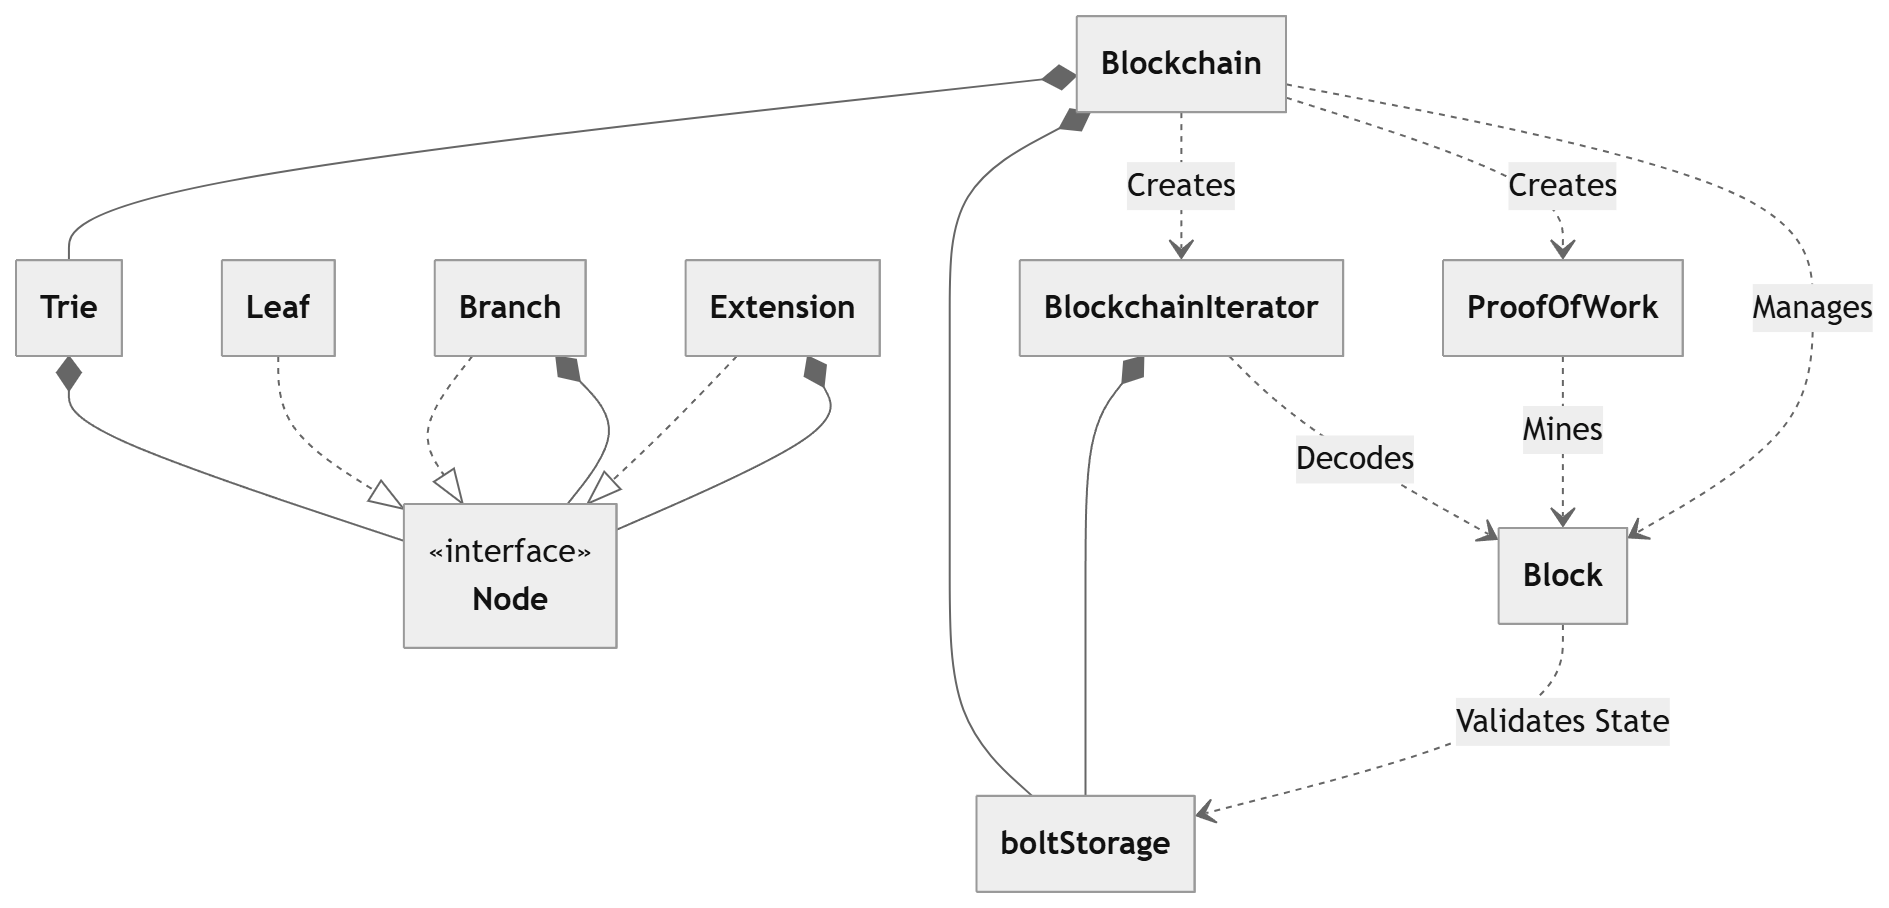
\includegraphics[width=1\textwidth]{simplest_diagram.png}
		\caption{Class diagram}
		\label{fig:class_diagram}
	\end{figure*}
	
	\FloatBarrier
	
	\subsection{Class Diagram}
	
	\begin{itemize}
		\item \textbf{Blockchain.} Acts as the primary entry point, maintaining a direct strong composition relationship over the active \texttt{Trie} model and overseeing database transactions.
		\item \textbf{boltStorage.} Utilizes an instance of \texttt{boltStorage} to write data into two buckets (\texttt{"blocks"} and \texttt{"tries"}).
		\item \textbf{BlockchainIterator.} Manages a strong composition relationship back to the database, tracking byte-serialized headers backwards via the block's embedded \texttt{PrevBlockHash} hash pointer.
		\item \textbf{Proof of Work.} Responsible of performing the block mining process, trying to achieve a hash lower than a specific target produced by a certain difficulty.
		\item \textbf{Block.} It contains the unique information for identification purpose and also the hash of previous block to grant immutability and enable block iteration over the chain.
		\item \textbf{Trie.} Data structure used to store pair key-values, in this case strings transformed to bytes. The trie only contains the root node, and you can visit all nodes that belong to the trie recursively starting from the root node. A "Node" is a Go interface that could be either a "Leaf", "Branch" or "Extension" classes which functionalities have been explained previously.
	\end{itemize}
	
	A complete version of the class diagram can be found in the github repository \cite{jowy-ti_dsproject}
	
	\subsection{System Architecture}
	
	The architecture has three main layers which can be well differentiated in the Figure \ref{fig:architecture}. Responsibilities of each layer are the following:
	
	\begin{enumerate}	
		\item \textbf{Client Interface.} Is the only part of the program that directly interacts with the user and calls the appropriate functions of the Blockchain core logic layer to perform the actions. This layer is a CLI and has some features like auto-complete and commands usage help.
		
		\item \textbf{Blockchain core logic and consensus layer.} Provides the core logic that can perform four main actions:
		
		\begin{itemize}
			\item \textbf{Chain validation.} Performed every time a block wants to be added to assure that the chain is valid and not a fraud.
			\item \textbf{Trie creation.} Process of adding elements to a trie till is decided it is completed.
			\item \textbf{Block assembly.} Once the trie is built a block is initialized with its respective data and the first value of the nonce "0".
			\item \textbf{Block mining.} Finally, this step performs Proof of Work (PoW), iterating nonce values till it produces a hash value lower than a target. Once the a block has been mined successfully, it is sent to the next layer to be stored.
		\end{itemize}
		
		\item \textbf{Persistent storage DB.} Its purpose is to manage the interaction with database (BoltDB) retrieving or storing the information. The database is divided into two buckets for the different kind of data that this program handles (trie and block data).	
	\end{enumerate}	
	
	\begin{figure}[htbp]
		\centering
		\includesvg[width=1\linewidth]{architecture.svg}
		\caption{Architecture}
		\label{fig:architecture}
	\end{figure}
	
	\section{Critical Trade-offs and Vulnerabilities}
	
	\subsection{Storage Write Amplification}
	Because the MPT resets cleanly at the termination of each block cycle, the MPT acts as an block isolated ledger rather than a persistent world state. However, during data insertion phases, updating a leaf node alters its hash signature, breaking its parent branch hash. This domino effect scales recursively up to the tree head, generating high disk-write workloads proportional to trie depth.

	\subsection{Vulnerability Assessment}
	\begin{itemize}
		\item \textbf{Lack of Authorization and Signature Verification:} Payloads are processed as arbitrary data strings. The missing implementation of public-key cryptography (such as ECDSA or Ed25519 digital signatures) creates a vulnerability where transaction ownership or authenticity cannot be validated.
		\item \textbf{Exposure to State Bloat DoS Attacks:} The absence of an economic gas or processing fee model allows a malicious agent to execute infinite value insertions for free, risking host disk space exhaustion.
	\end{itemize}
	
	\section{Conclusion and Future Work}
	This paper successfully presented a modular, clean research framework implemented in Go with debugging tools and experimental tests that successfully isolates and studies Proof-of-Work constraints and specialized Merkle Patricia Trie behaviors facilitating newcomers understand better this concepts and extending functionalities. By mapping paths strictly via content hashes, the MPT architecture successfully optimizes out branch value requirements. Future milestones will focus on transitioning this block-centric log structure into a cumulative, rolling world-state engine by persisting root hash variables across block headers, replacing the GOB encoder with a deterministic RLP framework, and establishing cryptographic signature enforcement mechanisms.
	
	\bibliographystyle{IEEEtran}
	\bibliography{references}
	
\end{document}